\documentclass[12pt, a4paper, landscape]{memoir}
\usepackage[margin=0pt]{geometry}
\usepackage[utf8]{inputenc}
\usepackage{babel}
\usepackage[T1]{fontenc}
\usepackage{adjustbox}
\usepackage{amsmath}

\usepackage{tikz}
\usepackage{url}
\graphicspath{ {./images/} }

\pagenumbering{gobble}

\begin{document}
	\vspace*{-0.8em}
	\begin{center}
		{\LARGE Pascalov trojuholník}\\[1em]
		\large
		\begin{vplace}[0.5]
		\begin{adjustbox}{max width=.95\paperwidth, max height=.95\paperheight}	
			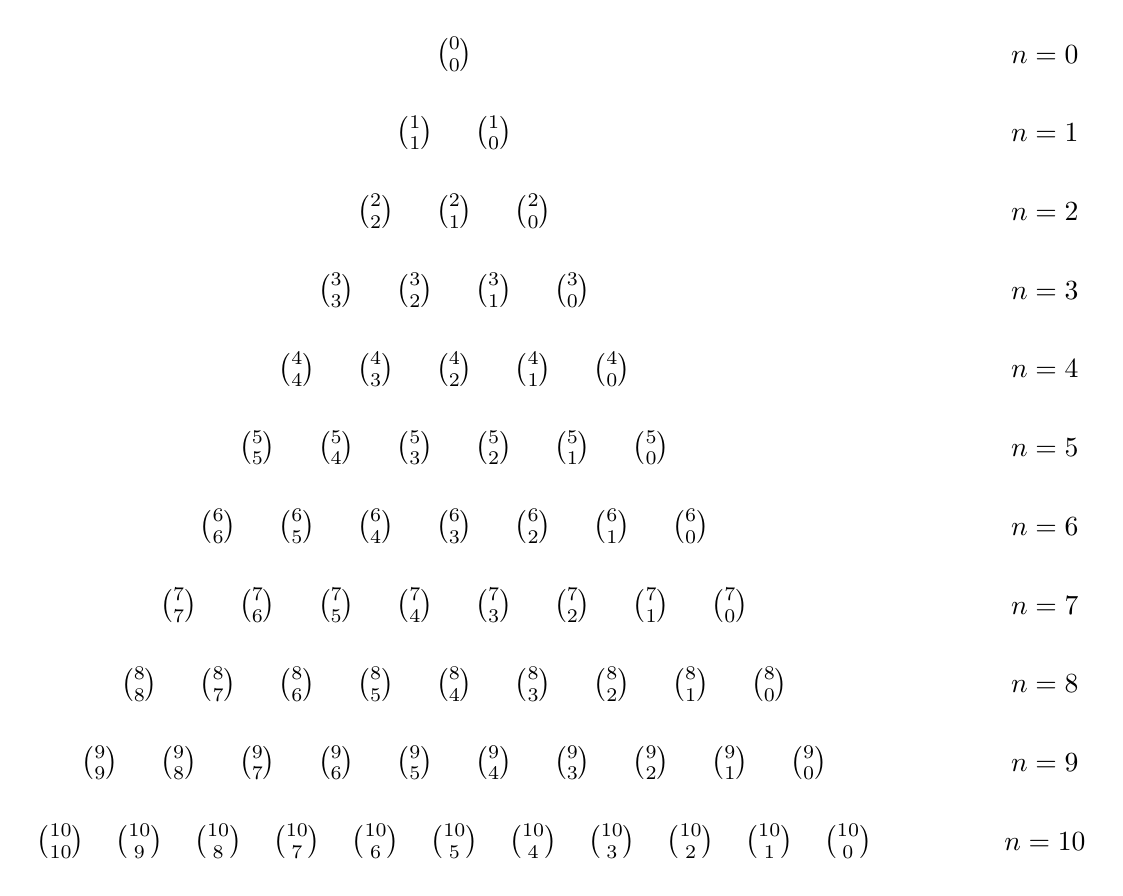
\begin{tikzpicture}
				\node at (-0.0, 0) {$0 \choose 0$};
\node at (7.5, 0) {$n = 0$};
\node at (0.5, -1) {$1 \choose 0$};
\node at (-0.5, -1) {$1 \choose 1$};
\node at (7.5, -1) {$n = 1$};
\node at (1.0, -2) {$2 \choose 0$};
\node at (-0.0, -2) {$2 \choose 1$};
\node at (-1.0, -2) {$2 \choose 2$};
\node at (7.5, -2) {$n = 2$};
\node at (1.5, -3) {$3 \choose 0$};
\node at (0.5, -3) {$3 \choose 1$};
\node at (-0.5, -3) {$3 \choose 2$};
\node at (-1.5, -3) {$3 \choose 3$};
\node at (7.5, -3) {$n = 3$};
\node at (2.0, -4) {$4 \choose 0$};
\node at (1.0, -4) {$4 \choose 1$};
\node at (-0.0, -4) {$4 \choose 2$};
\node at (-1.0, -4) {$4 \choose 3$};
\node at (-2.0, -4) {$4 \choose 4$};
\node at (7.5, -4) {$n = 4$};
\node at (2.5, -5) {$5 \choose 0$};
\node at (1.5, -5) {$5 \choose 1$};
\node at (0.5, -5) {$5 \choose 2$};
\node at (-0.5, -5) {$5 \choose 3$};
\node at (-1.5, -5) {$5 \choose 4$};
\node at (-2.5, -5) {$5 \choose 5$};
\node at (7.5, -5) {$n = 5$};
\node at (3.0, -6) {$6 \choose 0$};
\node at (2.0, -6) {$6 \choose 1$};
\node at (1.0, -6) {$6 \choose 2$};
\node at (-0.0, -6) {$6 \choose 3$};
\node at (-1.0, -6) {$6 \choose 4$};
\node at (-2.0, -6) {$6 \choose 5$};
\node at (-3.0, -6) {$6 \choose 6$};
\node at (7.5, -6) {$n = 6$};
\node at (3.5, -7) {$7 \choose 0$};
\node at (2.5, -7) {$7 \choose 1$};
\node at (1.5, -7) {$7 \choose 2$};
\node at (0.5, -7) {$7 \choose 3$};
\node at (-0.5, -7) {$7 \choose 4$};
\node at (-1.5, -7) {$7 \choose 5$};
\node at (-2.5, -7) {$7 \choose 6$};
\node at (-3.5, -7) {$7 \choose 7$};
\node at (7.5, -7) {$n = 7$};
\node at (4.0, -8) {$8 \choose 0$};
\node at (3.0, -8) {$8 \choose 1$};
\node at (2.0, -8) {$8 \choose 2$};
\node at (1.0, -8) {$8 \choose 3$};
\node at (-0.0, -8) {$8 \choose 4$};
\node at (-1.0, -8) {$8 \choose 5$};
\node at (-2.0, -8) {$8 \choose 6$};
\node at (-3.0, -8) {$8 \choose 7$};
\node at (-4.0, -8) {$8 \choose 8$};
\node at (7.5, -8) {$n = 8$};
\node at (4.5, -9) {$9 \choose 0$};
\node at (3.5, -9) {$9 \choose 1$};
\node at (2.5, -9) {$9 \choose 2$};
\node at (1.5, -9) {$9 \choose 3$};
\node at (0.5, -9) {$9 \choose 4$};
\node at (-0.5, -9) {$9 \choose 5$};
\node at (-1.5, -9) {$9 \choose 6$};
\node at (-2.5, -9) {$9 \choose 7$};
\node at (-3.5, -9) {$9 \choose 8$};
\node at (-4.5, -9) {$9 \choose 9$};
\node at (7.5, -9) {$n = 9$};
\node at (5.0, -10) {$10 \choose 0$};
\node at (4.0, -10) {$10 \choose 1$};
\node at (3.0, -10) {$10 \choose 2$};
\node at (2.0, -10) {$10 \choose 3$};
\node at (1.0, -10) {$10 \choose 4$};
\node at (-0.0, -10) {$10 \choose 5$};
\node at (-1.0, -10) {$10 \choose 6$};
\node at (-2.0, -10) {$10 \choose 7$};
\node at (-3.0, -10) {$10 \choose 8$};
\node at (-4.0, -10) {$10 \choose 9$};
\node at (-5.0, -10) {$10 \choose 10$};
\node at (7.5, -10) {$n = 10$};
			\end{tikzpicture}
		\end{adjustbox}
		\end{vplace}
	\end{center}
\end{document}
